\chapter{Dual-Phase Far Detector Technology}
\label{ch:exec-dp}

\textit{This chapter provides a brief introduction to the dual-phase far detector technology.  The text below closely follows that found in the introductory chapter of Volume~\volnumberdp{}, \voltitledp{}, where many more details may be found.}


\section{Overview}
\label{sec:dp-execsum-introduction}


\dword{dune}'s rich physics program, with discovery potential for \dword{cp} violation in the neutrino sector and its capability to make significant observations of nucleon decay and astrophysical events is enabled by the exquisite resolution of the \dword{lartpc} detector technique, which the \dword{dp} design further augments relative to the \dword{sp} design. 
In a \dword{dpmod} ionization charges drift vertically in \dword{lar} and are transferred
into a layer of gas above the liquid. This design allows for a single, fully homogeneous \dword{lar} volume, offering a much longer drift length and reducing  the quantity of nonactive materials in the \dword{lar}.
The design also improves the \dword{s/n} ratio in the charge readout, reducing the threshold for the smallest observable signals, while also achieving a finer readout granularity.  
Other advantages of the \dword{dp} design include accessible readout electronics and fewer detector components, reducing both costs and installation logistics.
  
The operating principle of a \dword{dp} \dword{lartpc}, illustrated in Figure~\ref{fig:figure-label-DPprinciple}, is very similar to that of the \dword{sp} design (Figure~\ref{fig:spLArTPC}).  Charged particles that traverse the active volume of the \dword{lartpc} ionize the medium while also producing scintillation light. The ionization electrons drift along an \efield towards a segmented anode where they deposit their charge. The precision tracking and calorimetry offered by the \dword{dp} technology provides excellent capabilities for identifying interactions of interest while mitigating sources of background.  

\begin{dunefigure}[Principle of the \dual readout]{fig:figure-label-DPprinciple}{Principle of the DP readout.}
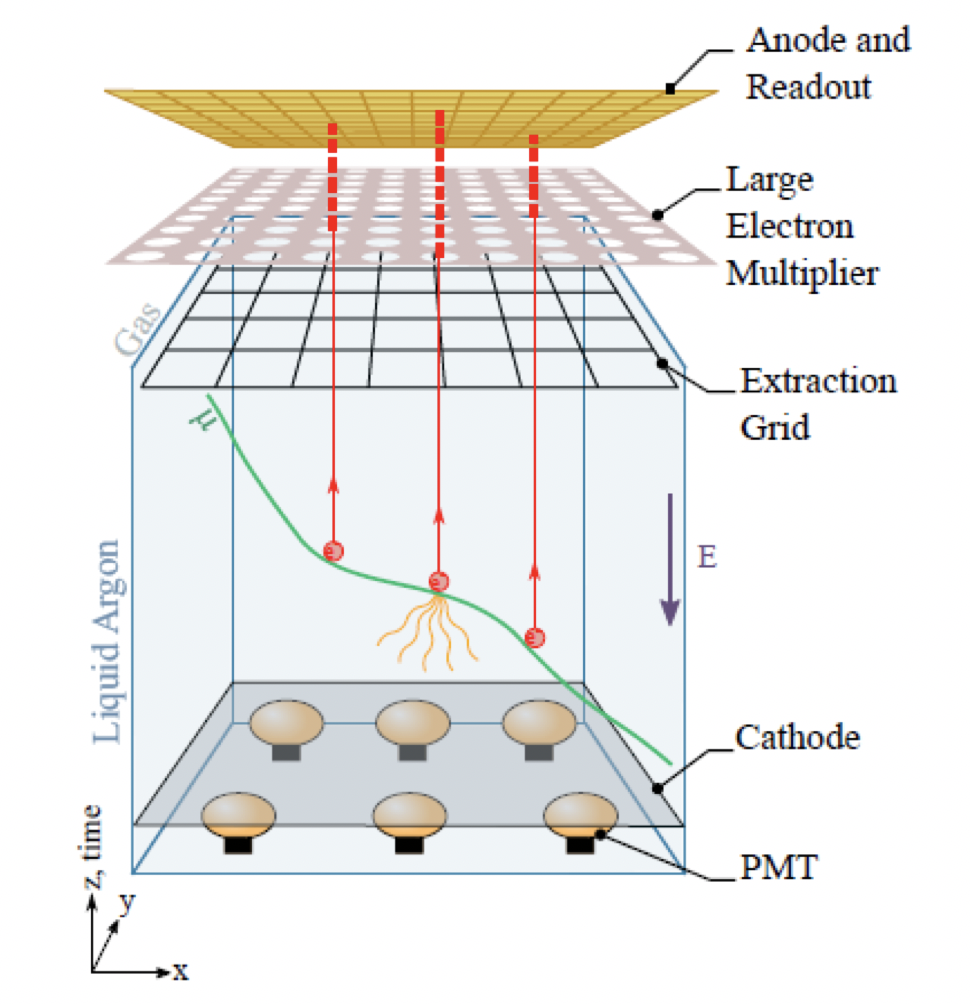
\includegraphics[width=0.6\textwidth]{dualphase-principle}
\end{dunefigure}

The argon scintillation light, at a wavelength of  \SI{127}{nm}, is deep in the UV spectrum. It is recorded by an array of \dwords{pmt} located below the cathode at the bottom of the cryostat.  The \dwords{pmt}, coated with a wavelength-shifting material, shift the light closer to the visible spectrum and record the time and pulse characteristics of the incident light.

Two key factors affect the performance of the \dword{lartpc}, argon purity and noise.  The \dword{dp} and \dword{sp} designs have slightly different purity requirements to cope optimally with the different drift lengths. We express the purity level in terms of electron lifetime: a minimum of \SI{5}{ms} for \dword{dp} versus \SI{3}{ms} for \dword{sp}. In both cases the levels of electronegative contaminants in the \dword{lar} (e.g., oxygen and water) must remain 
at \dword{ppt} levels.  
To clearly discern the drifting electrons over the baseline of the electronics, the \dword{tpc}  electronic readout noise must be kept very low. This requires use of low-noise cryogenic electronics. 
Amplification of the electron signal in the gas phase mitigates the potential effect of both factors on the performance.  On the other hand, due to the longer drift length, the \dword{dp} design requires a higher voltage (up to \SI{600}{kV}) on the cathode. \fixme{how does this affect the purity and noise?}



%%%%%%%%%%%%%%%%%%%%%%%%%%%%%%%%%%%%%%%%%%%%%%%%%%%%%%%%%%%%%%%%%%%%
\section{Overview of Dual-Phase Design}
\label{sec:dp-execsum-description}

The \dword{dpmod} features a  \dpactivelarmass{} active mass \dword{lartpc}, of dimensions (LWH) \dptpclen by \dptpcwdth by \tpcheight{}. It includes all associated cryogenics, electronic readout, computing, and safety systems. The module is built as a single active volume, with the anode at the top, the cathode near the bottom, and an array of \dwords{pd} underneath the cathode. The active volume (see Figure~\ref{fig:DPdet1}) is surrounded by a \dword{fc}. 
The \dword{dp} design maximizes the active volume within the confines of the membrane cryostat while minimizing dead regions and the presence of dead materials in the drift region.  The detector elements are all modular to facilitate production and to allow for transport underground.


The key differentiating concept of the \dword{dp} design is the amplification of the ionization signal in an ``avalanche'' process.  Ionization electrons drift upward toward an extraction grid situated just below the liquid-vapor interface. After reaching the grid, an \efield stronger than the drift field extracts the electrons from the liquid upward into the ultra-pure argon gas. 
Once in the gas, the electrons encounter detectors, called \dwords{lem}, that have a micro-pattern of high-field regions in which the electrons are greatly amplified (via avalanches caused by Townsend multiplication). 
The amplified charge is collected on an anode. The use of avalanches to amplify the charges in the gas phase increases the \dword{s/n} ratio by at least
a factor of ten, with the goal of achieving a gain of about 20, which will significantly improve the
event reconstruction quality.



The modular extraction grids, \dwords{lem}, and anodes are assembled into three-layered sandwiches with precisely defined inter-stage distances and inter-alignment,  which are then connected together horizontally into modular detection units that are \num{9}~m$^2$. These composite detection units, called \dwords{crp}, are discussed in Section~\ref{sec:dp-execsum-crp}.
A \dword{crp} provides an adjustable charge gain and two independent, orthogonal readout views, each with a pitch of \dpstrippitch. It collects the charge projectively, with practically no dead region. Together, the time information  ($t_0$) from the \dword{lar} scintillation readout and the  \threed track imaging of the \dwords{crp} provide $dE/dx$ information.  

Slow-control \fdth{}s,  one per \dword{crp}, are used for level meter and temperature probe readout,  for pulsing calibration signals, and to apply \dword{hv} bias on the two sides of the \dwords{lem} and on the extraction grid. Calibration and \dword{cisc} systems for the \dword{sp} and \dword{dp} technologies have been designed jointly, and are discussed in Sections~\ref{sec:exec-sp-calibration} and~\ref{sec:dp-execsum-sc}, respectively.

Signals in each \dword{crp} unit are collected via three \dwords{sftchimney} on the roof of the cryostat that house the \dword{fe} cards with the (replaceable) cryogenic \dword{asic} amplifiers.  The only active electronics elements inside the cryostat are the \dword{pmt} bases.  Each \dword{sftchimney} is coupled to a \dword{utca} crate to provide signal digitization and \dword{daq}. These crates are connected  via optical fiber links to the \dword{daq} back-end. The total number of readout channels  per \nominalmodsize module is \dpnumcrpch.
%%

Figure~\ref{fig:DPdet1} shows the \dword{dpmod}'s main components.

\begin{dunefigure}[Diagram of a \dshort{dpmod}]{fig:DPdet1}
  {A \dword{dpmod} with cathode, \dwords{pmt}, \dword{fc}, and anode plane with \dwords{sftchimney}.}
  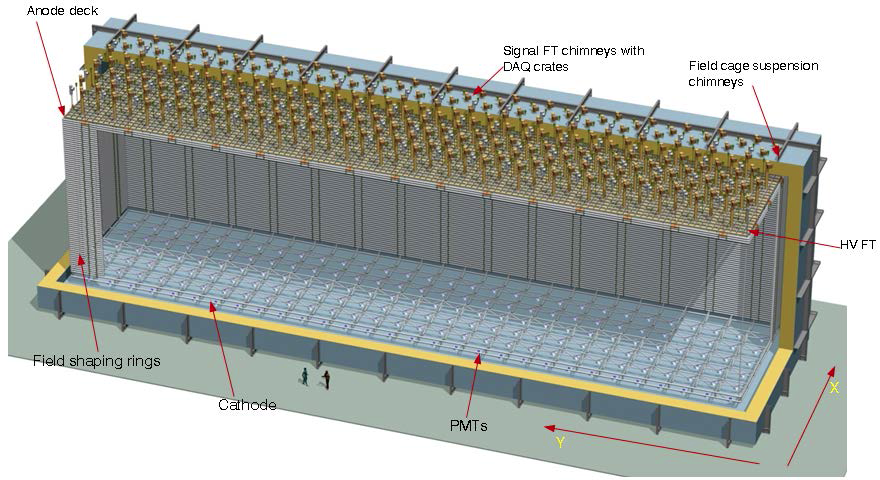
\includegraphics[width=0.9\textwidth]{DUNE-CDR-detectors-volume-optim.png}
\end{dunefigure}


The number of components and corresponding parameters for a \dpactivelarmass \dword{dpmod} are summarized in Table~\ref{tab:DP_numbers}.

\begin{dunetable}[\dshort{dpmod} component quantities and parameters]{ll}{tab:DP_numbers}{\dshort{dpmod} component quantities and parameters.}  Component & Value    \\ \toprowrule
Anode plane size & W = \dptpcwdth, L = \dptpclen \\ \colhline
\dshort{crp} unit size & W = \SI{3}{m}, L = \SI{3}{m}  \\ \colhline
\dshorts{crp} & \num{4}\,$\times$\,\num{20} = \dptotcrp \\ \colhline
\dshort{crp} channels & \dpnumcrpch  \\ \colhline 
\dshort{lem}-anode sandwiches per \dword{crp} unit & \dpswchpercrp \\ \colhline 
\dshort{lem}-anode sandwiches (total) & \dpnumswch \\ \colhline
\dshorts{sftchimney} per \dword{crp} unit & \num{3} \\ \colhline
\dshorts{sftchimney} & \num{240} \\ \colhline
Charge readout channels per \dword{sftchimney} & \num{640}  \\ \colhline
Charge readout channels (total) & \dpnumcrpch \\ \colhline
Suspension \fdth per \dword{crp} unit & \num{3}  \\ \colhline
Suspension \fdth{}s  (total)& \num{240}  \\ \colhline
Slow control \fdth{}s   (total)& \num{80} \\ \colhline
\dshort{hv} \fdth & \num{1}  \\ \colhline
Nominal drift \efield & \SI{0.5}{kV/cm}  \\ \colhline
Nominal/target \dshort{hv} for vertical drift & \dpnominaldriftfield{}/\dptargetdriftvoltpos \\ \colhline
\dshort{fc} voltage degrader resistive chains & \num{12} \\ \colhline
\dshort{fc} cathode modules & \num{15}  \\ \colhline
\dshort{fc} rings & \num{199}     \\ \colhline
\dshort{fc} modules (\SI{4}{m}$\times$\SI{12}{m}) & \num{36}  \\ \colhline
\dshorts{pmt}  & \dpnumpmtch (\num{1}/m$^2$) \\  \colhline
\dshort{pmt} channels & \dpnumpmtch  \\ 
\end{dunetable}


%%%%%%%%%%%%%%%%%%%%%%%%%%%%%%%%%%%
\section{Charge Readout Planes}
\label{sec:dp-execsum-crp}

The  collection, amplification, and readout components of the \dword{tpc} are combined into  layered modules called \dwords{crp}. The charge is collected in a finely segmented readout anode plane at the top of the gas volume and fed to the \dword{fe} readout electronics. The  \dword{crp}'s amplification components, the \dwords{lem}, are horizontally oriented \SI{1}{mm}-thick printed circuit boards (\dwords{pcb}) with electrodes on the top and bottom surfaces.  
The \dword{crp} structure also integrates the immersed extraction grid, which is an array of $x$- and $y$-oriented stainless steel wires, \SI{0.1}{mm} in diameter, with a \dpstrippitch pitch. Figure~\ref{fig:CRP_struct} shows the thicknesses and possible biasing voltages for the different \dword{crp} layers.

Each \dword{crp} is made up of several independent \num{0.5}\,$\times$\,\SI{0.5}{m$^2$} units, each of which is composed  of a \dword{lem}-anode ``sandwich.''  
The anode is a two-dimensional (\twod) \dword{pcb} with two sets of \SI{3.125}{mm}-pitch gold-plated copper strips that provide the $x$ and $y$ coordinates (and thus two views) of an event. Both the \dwords{lem} and anodes are produced in units of $50 \times 50\, $cm$^2$. 
The \dwords{crp} are embedded in a mechanically reinforced frame of \frfour and iron-nickel invar alloy. 




An extraction efficiency of \num{100}\,\% of the electrons from the liquid to the gas phase is achieved with an \efield of the order of \SI{2}{kV/cm} across the liquid-gas interface, applied between the  extraction grid immersed in the liquid and charge amplification devices situated above, in the argon gas. 

\begin{dunefigure}[Thicknesses and HV values for electron extraction from liquid to gaseous Ar]{fig:CRP_struct}
{Thicknesses and \dword{hv} values for electron extraction from liquid to gaseous argon, their  multiplication by \dwords{lem}, and their collection on the $x$ and $y$ readout anode plane. The \dword{hv} values are indicated for a drift field of \SI{0.5}{kV/cm} in \dword{lar}.}
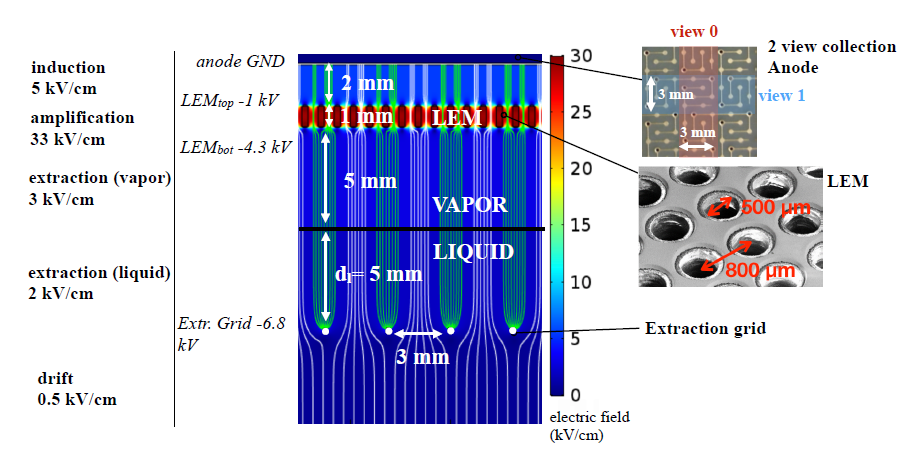
\includegraphics[width=0.8\textwidth]{CRP_gaps.png}
\end{dunefigure}

The \dwords{lem} are drilled through with many tiny holes (these are the high-field regions), that collectively form a micro-pattern structure. When a \SI{3}{kV} potential difference is applied across the a \dword{lem}'s electrodes, the high \efield (\SI{30}{kV/cm}) produces avalanches (via Townsend multiplication) that amplify the ionization electrons.  


Each \dword{crp} is independently suspended by three stainless-steel ropes linked to the top deck of the cryostat. This suspension system allows adjustment of the \dword{crp} height and level such that it remains parallel to the \dword{lar} surface and the extraction grid remains immersed.   

%%%%%%%%%%%%%%%%%%%%%%%%%%%%%%%%%%%
\section{Cathode, Field Cage, and HV System}
\label{sec:dp-execsum-cathode}

The drift field (nominal: E ${\simeq}$ \SI{0.5}{kV/cm}, minimum: E ${\simeq}$ \SI{0.25}{kV/cm}) inside the fully active \dword{lar} volume is produced by applying \dword{hv} to the cathode plane at the bottom of the cryostat and is kept uniform by the \dword{fc}, a stack of \num{199} equally spaced, field-shaping electrodes. 
These electrodes are set to linearly decreasing voltages starting from the cathode voltage at the bottom of the \dword{detmodule} to almost ground potential at the level of the \dword{crp}. 


The cathode plane  is suspended from the \dword{fc} and hangs near the  bottom of the cryostat. It consists of 15 adjacent \SI{4x12}{m} 
modules to span the \dptpclen length of \dword{dpmod}. 

As shown in  Figure~\ref{fig:dp-execsum-dune-dp-cathode}, each cathode module is constructed of two \SI{12}{m} long trusses made from thin-walled stainless steel tubes with an  outer diameter of approximately \SI{50}{mm}. 


\begin{dunefigure}[A \dshort{dp} cathode module]{fig:dp-execsum-dune-dp-cathode}
{Illustration of a \dword{dp} cathode module.  It is constructed using a pair of stainless steel trusses (blue) as the framework with an array of coated \dword{frp} rods. 
The lower-left inset shows the resistive interconnections and the lifting tab on the cathode truss structure. The upper-right inset is shows the resistive union.}
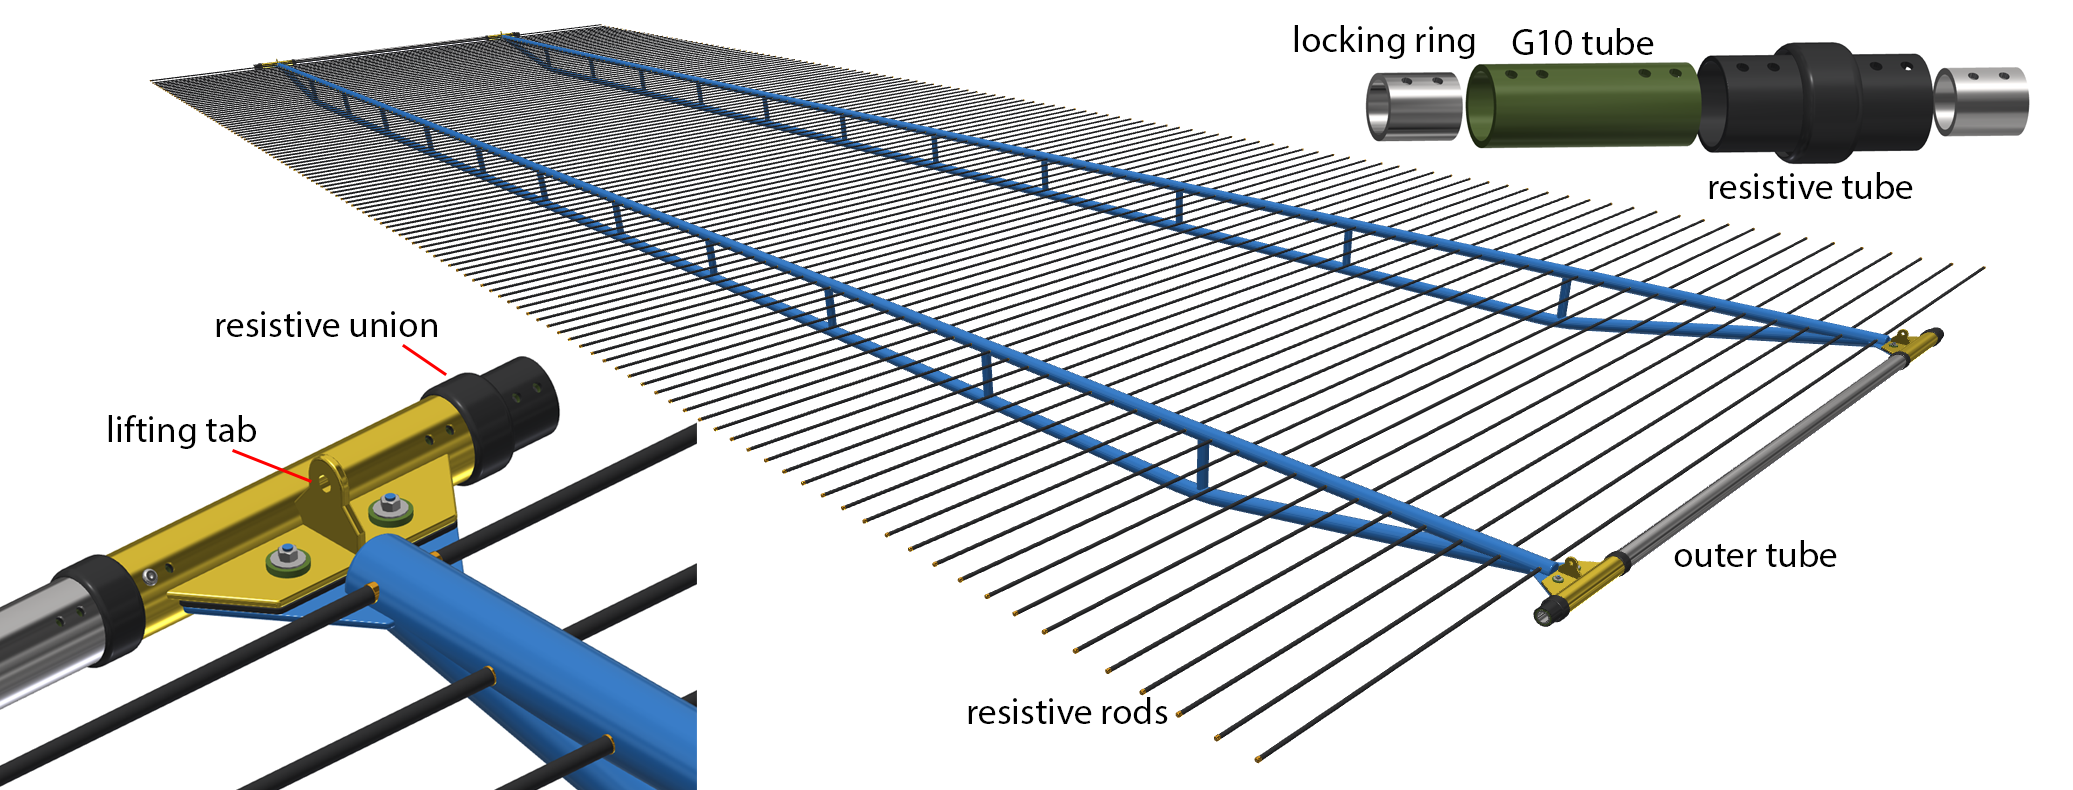
\includegraphics[width=0.9\textwidth]{DP_HVS_cathode_module.png}
\end{dunefigure}

A set of 80 \SI{3x3}{m} \dword{gg} modules, standing on the cryostat floor, are installed to protect the array of \dwords{pmt} against any electric discharge from the cathode.




%%%%%%%%%%%%%%%%%%%%%%%%%%%%%%%%%%%
\section{Readout Electronics and Chimneys}
\label{sec:dp-execsum-electronics}

The electrical signals from the collected charges are passed to the outside of the cryostat via a set of dedicated \dwords{sftchimney}, tightly-fit pipes that penetrate the top layer of the cryostat insulation, and are therefore exposed to cryogenic temperatures at their lower ends and to room temperature above the cryostat. They are filled with nitrogen gas and closed at the top and  bottom by ultra-high-vacuum flanges (warm and cold).  

The cryogenic analog \dword{fe} electronics cards, mounted on \SI{2}{m} long blades that slide on lateral guides that are integrated into the mechanical structure of the \dword{sftchimney}, are installed at the bottom of the chimney and plugged into the top side of the cold flange. 
This arrangement allows access to and replacement of the cards from the outside. 
 The warm flange connects the analog differential signals to external digitization cards. In the other direction, it distributes the \dword{lv} and slow control signals to the \dword{fe} electronics.  The chimneys act also as Faraday cages, preventing the analog \dword{fe} electronics  from picking up possible noise from the digital electronics.   
 
The \dword{fe} cards are based on the analog cryogenic preamplifiers implemented in \dword{cmos} \dword{asic} circuits designed for high integration and large-scale affordable production. 
The \dword{asic} for the \dword{dpmod} circuits have been specially engineered to match the \dword{dpmod}'s signal dynamics. Inside the \dwords{sftchimney}, the cards are actively cooled to a temperature of approximately \SI{110}{K}.  The bottom sides of the cold flanges connect to  \dwords{crp} via flat \SI{0.5}{m} long cables intended to minimize the input capacitance to the preamplifiers. Each \dword{sftchimney} collects \num{640} readout channels. 

The digital electronics for the charge digitization system is installed on the cryostat roof. 
This makes it possible to use common design standards and benefit from commercially supported low-cost, high-speed networking technologies, such as \dword{utca}, which is used in the telecommunications industry.

Digitization cards in the \dword{amc} format read \num{64} channels per card. Each \dword{amc} card can digitize \num{64} channels at \SI{2.5}{MHz} and compress and transmit this continuous data stream, without zero-skipping, over a network link operating at \SI{10}{Gbit/s}. Lossless data compression is particularly effective thanks to the high \dword{s/n} ratio  of \dword{dp}, which limits noise contributions at the level of one \dword{adc} count. Each \dword{sftchimney} is coupled to a \dword{utca} crate that holds \num{10} \dword{amc} digitization cards and can therefore read  \num{640} channels. The \dword{amc} cards  transmit the data to the \dword{daq} back-end. A total of \num{240} \dword{utca} crates are required for reading the entire \dword{detmodule}.  

The light-readout digitization system uses \dword{utca} \dword{amc} card design derived from that of the charge readout system, but that implements a circuitry based on the \dword{catiroc} \dword{asic} to trigger the readout. 

\fixme{not sure about next pgraph...  it's not clear to me -- is it synchronization between the tpc and pd readout electronics? is the info useful?}

The timing synchronization is based on the \dword{wr} standard. Specifically developed timing \dword{mch} connected to a \dword{wr} network ensures the distribution of clock, absolute timing, and trigger information on the backplane of the \dword{utca} crates. The \dword{wrmch} are connected via \SI{1}{Gbit/s} optical fibers to a system of \dword{wr} switches that interconnect the \dword{wr} network. This ensures that the digitization performed by the various \dword{amc} cards is completely aligned; it also refers to the absolute UTC time. 

%The \dword{wrgm} switch is connected to a GPS disciplined oscillator unit providing absolute time and the clock frequency reference to the system. The timing system includes \num{16} \dword{wr} switches and \num{240} (charge readout) + \num{5} (light readout) \dword{mch} units.    




%%%%%%%%%%%%%%%%%%%%%%%%%%%%%%%%%%%
\section{Photon Detection System}
\label{sec:dp-execsum-pd}

The \dword{pds} is based on an array of \dwords{pmt} uniformly distributed below the cathode. 
The \dwords{pmt} have a \dword{tpb} coating on the photocathode's external glass surface that shifts the scintillation light from deep UV to visible light. The \dwords{pmt}  sit on the corrugated membrane cryostat floor, on 
mechanical supports that do not interfere with the membrane thermal contraction. 
Figure \ref{fig:dp-execsum-dppd_3_2} shows the \dword{pmt} with its support base attached to the bottom of the \dword{pddp} cryostat (Section~\ref{sec:exec:overall:pdune}).

\begin{dunefigure}[A Hamamatsu R5912-MOD20 \dshort{pmt} in \dshort{pddp}]{fig:dp-execsum-dppd_3_2}
{Picture of the cryogenic Hamamatsu R5912-MOD20 \dword{pmt} fixed on the membrane floor of \dword{pddp}. The optical fiber of the calibration system is also visible.}
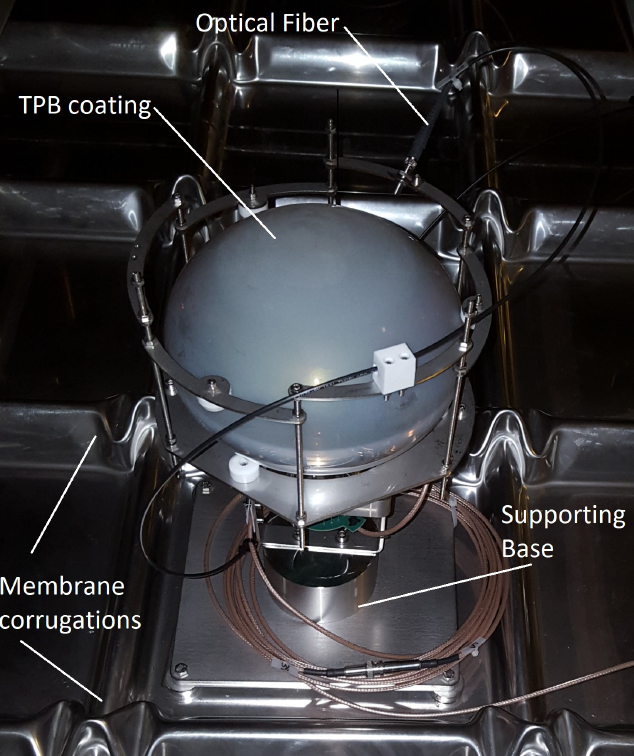
\includegraphics[width=0.42\textwidth]{dp-execsum-pmt1}
\end{dunefigure}

In order to improve the light yield uniformity for signals generated in the top part of the drift volume a system of reflective panels with WLS coating is integrated on the  \dword{fc} walls.


%%%%%%%%%%%%%%%%%%%%%%%%%%%%%%%%%%%
\section{Data Acquisition}
\label{sec:dp-execsum-daq}

The \dword{daq} systems for both the \dword{sp} and \dword{dp} technologies have been designed jointly and are identical except for the architecture of the detector readout electronics.  The output format of the generated data is common, and both are synchronized to the same global clock signals. The shared \dword{daq} design is introduced in Section~\ref{sec:exec-sp-daq}.

The \dword{dp} readout architecture can be organized into \num{20} regions of interest (\dwords{roi}). %, each similar to the \dword{pddp} back-end architecture. 
Triggers are searched on the level-1 event builder machines, interconnecting multiple \dword{utca} crates, on a sliding windows of \SI{10}{s} contained in the event builder RAM.
Figure~\ref{fig:dp-execsum-daq-interface-scheme} illustrates the \dword{dp} readout architecture (bottom) and its interface to the \dword{daq} system.
  
  \fixme{I do not find similar language in the DP DAQ chapter. Just sayin'.}

\begin{dunefigure}[Interface of DP TPC electronics to DAQ]{fig:dp-execsum-daq-interface-scheme}
{Schematic illustration of the interface of \dword{dp} \dword{tpc} electronics to \dword{daq}.}
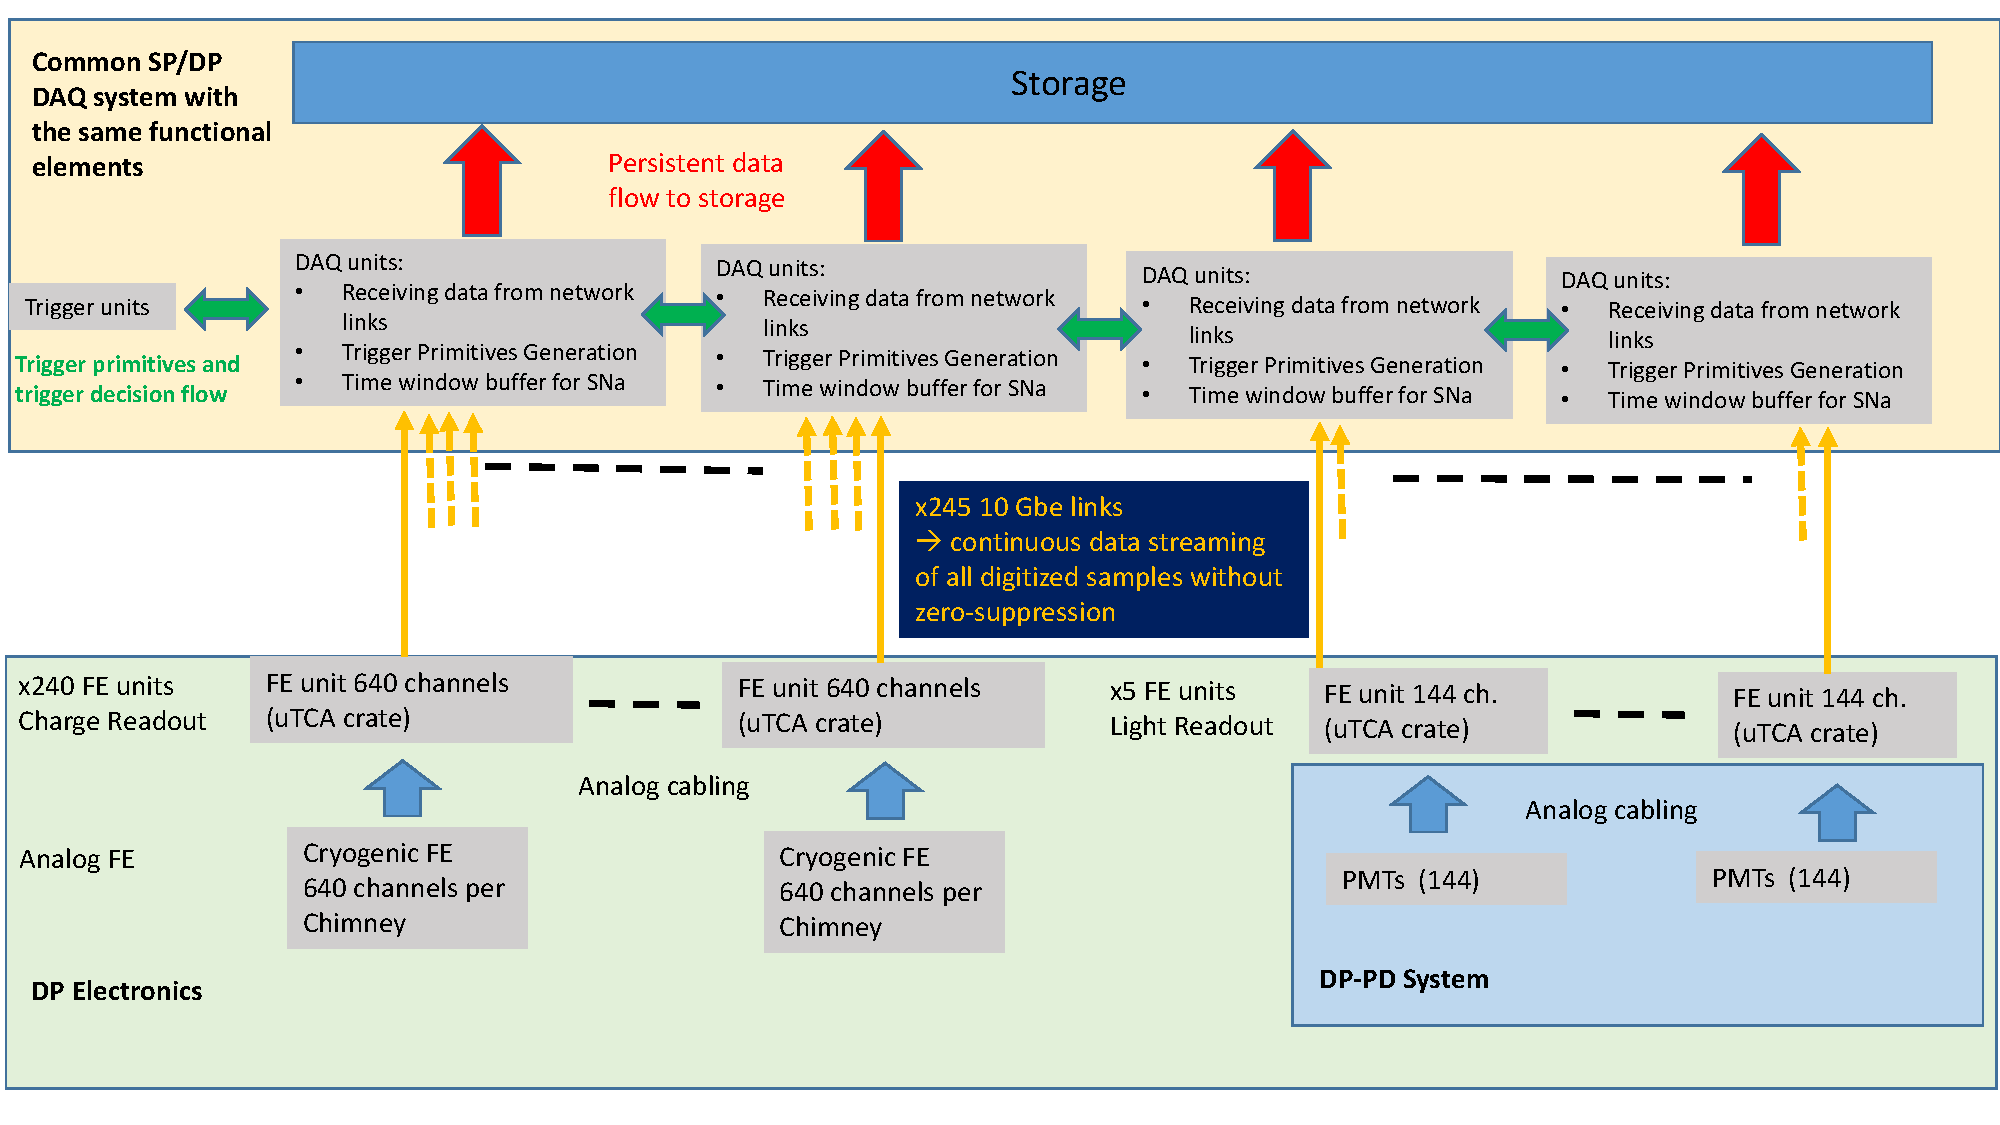
\includegraphics[width=0.95\textwidth]{dp-tpcelec-daq-interface-scheme}
\end{dunefigure}

